\documentclass[a4paper,10pt]{scrartcl}
%encodings
\usepackage[utf8]{inputenc}
\usepackage[english]{babel}
\usepackage[T1]{fontenc}
%colors, hyperrefs
\usepackage{color}
\usepackage{url}
\usepackage[pdftex,pdfauthor={J\"org Behrmann, Anika Haller},pdftitle={Ma12: Magneto-optical Kerr-effect and Magnetic Anisotropy}]{hyperref}
%figures and subfigures
\usepackage[pdftex]{graphicx}
\usepackage{subfigure}
%better tables
\usepackage{tabularx}
\usepackage{booktabs}
\usepackage{multirow}
%math stuff
\usepackage{amsmath}
\usepackage{amsthm}
\usepackage{amsfonts}
\usepackage{IEEEtrantools}
\usepackage[square,comma,numbers,sort&compress]{natbib}
%shiny stuff
\usepackage[babel]{microtype}
\DisableLigatures{encoding=T1,family=tt*}

\usepackage{textcomp}

\begin{document}

\title{Low Energu Electron Diffraction (LEED)}
\author{J\"org Behrmann\footnote{behrmann@physik.fu-berlin.de} \qquad Anika Haller\footnote{halleran@zedat.fu-berlin.de}}
\date{31.10.2011}
\maketitle
\tableofcontents
\thispagestyle{empty}

\section{Introduction}

In 1924 Louis de Broglie proposed the Particle Wave duality impliying that particles could have wave-like characteristics. This was proofed in 1926 by Davisson and Germer, who used the wave-properties of electrons to study Ni crystals. 

Their work is ancestral to the Low Energy Electron Diffractio, which is a spectroscopic technique that is used to study crystal surfaces and substrates on surfaces. LEED came up in the 1960s because of the need ultra high vacuum (UHV) that is needed. Electrons are favorable for surface structure analysis because they are easier to produce than neutrons and are much more sensitive to surfaces than X-rays because of their very short mean free path in solids.

\subsection{Particle Wave Duality}

The wavelength of a particle is given by the de Broglie relation
\begin{equation}
\lambda = \frac{h}{p} = \frac{h}{\sqrt{2mE_{kin}}} \label{eq:broglie1}
\end{equation}
where h is Planck's constant. For an charged particle that is accelerated by the voltage $U$ this amounts numerically to
\begin{equation}
\lambda = 12.26 \mbox{\AA} \sqrt{\frac{\mbox{ev}}{E_{kin}}} = 12.26 \mbox{\AA} \sqrt{\frac{\mbox{eV}}{qE}} \label{eq:broglie}
\end{equation}
When the wavelength of a particle is approximately equal to the lattice constant it can be used to examine the surface. For acceleration voltages in the range between $50$ to $500\,$V an electron's wavelength will be between $0.5$ and $2\,$\AA. Relativistic corrections are not needed at this energies, because 
\begin{equation}
\frac{E_{kin}}{E_0}=\frac{eU}{mc^2} \approx 1\mbox{\textperthousand}
\end{equation}

\subsection{Diffraction}

\subsection{Far Field Approximation}

When a plane wave $Ae^{ikx}$ falls on a pointlike scatterer it becomes the source of radial waves of the form
\begin{equation}
\phi=\int dy J(y)\frac{e^{i|k||x-y|}}{|x-y|} A e^{iky}, \label{eq:scatter}
\end{equation}
where the integration is over the whole scatterer and $J(x)$ describes the the response of the medium. The above expression can be found by finding the Green's function to the wave equation.
\begin{equation}
\phi(x)=\frac{A}{R}e^{ik'x}\int dyJ(y)e^{i(k-k')y}  \label{eq:farfield}
\end{equation}
This formula is~\eqref{eq:scatter} in the far field approximation, i.e. far away from the scattering event, which is most certainly true for our experiment. Additionally we assumed that the incoming wave is not substantially altered by the scattering event. In quantum mechanics this is called the Born approximation; it neglects subsequent scattering, because they are of order $J^{2}(x)$, as is known from basic courses on scattering theory. This assumption is save if $J(x)$ is much smaller than one, i.e. weak scattering potentials.

Equation~\eqref{eq:farfield} tells us that what can be experimentally observed is basically the Fourier transform of the scattering potential. 

\subsection{The Reciprocal lattice, Laue condition and Bragg formula}

We will now assume a form for $J(x)$
\begin{equation}
J_{A}(x)=\sum_{r\in\mathbb{\mathbb{Z^{n}}}}\delta(x-A\cdot r) \label{eq:dirac}
\end{equation} 
where $A$ is the $n \times n$ matrix of unit vectors of the lattics and x and r are n-dimensional vectors in the lattice. Equation~\eqref{eq:dirac} is the n-dimensional Dirac lattice, which for example for $n=1$ is called a Dirac comb. 

A well-known theorem on Fourier transformation tells us that the Fourier transform of a lattice is again a lattice
\begin{equation}
J(k)=\sum_{g\in\mathbb{Z}^{n}}\delta(k-G \cdot g),\quad \mbox{with} \quad G=2\pi(A^{-1})^{T}=2\pi A^{-T}. \label{eq:recproc}
\end{equation}
$G$ is the so-called reciprocal lattice and $g$ are the reciprocal lattice vectors. We now need to identify $k$ in~\eqref{eq:recproc} with $k-k'$ in equation~\eqref{eq:farfield}. This gives us the Laue condition, which states that we observe a peak whenever $k-k'$ equals a reciprocal lattice vector. This can be visualized quite nicely with the Ewald construction that can be found in figure~\ref{fig:ewald}.

\begin{figure}
\centering
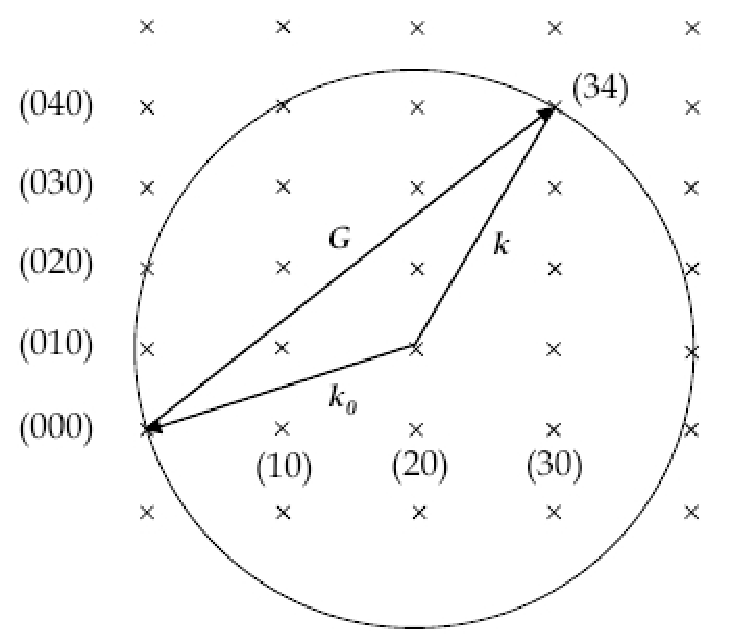
\includegraphics[scale=0.7]{img/ewald}
\caption{Ewald construction for the Laue condition. \label{fig:ewald}}
\end{figure}

The Laue condition is equivalent to the Bragg formula, which can be seen by squaring.
\begin{eqnarray}
g^{2} & = & k^{2}-2kk'+k'^{2} \\  
g^{2} & = & 2k^{2} (1-\cos \alpha) \\
g^{2} & = & 4k^{2}\sin^{2}\theta \label{eq:prebragg}
\end{eqnarray}
where $\alpha = 2 \theta$ is the angle between $k$ and $k'$. From the definition of the reciprocal lattice we can see that each reciprocal lattice vector is associated with a family of planes whose distance is given by $d=\tfrac{2\pi n}{|g|}$, where $n$ is a natural number so that $\tfrac{g}{n}$ is still a reciprocal lattice vector. Inserting this in the above equation we arrive at the Bragg formula
\begin{equation}
\lambda=2nd\sin\theta. \label{eq:bragg}
\end{equation}

In reality lattices will not be delta lattices. One will then need to add a structure factor to model the internal structure of a unit cell. Also peaks are not infinitely sharp delta peaks, so that a factor---the finite size factor---is needed to give them a finite width.

\subsubsection{A Two-Dimensional Lattice}

In the two-dimensional case the lattice matrix is given by 
\begin{equation}
A=\left(\begin{array}{cc}
a & 0\\
0 & a
\end{array}\right) \Longleftrightarrow G=\frac{2\pi}{a}\left(\begin{array}{cc}
1 & 0\\
0 & 1
\end{array}\right). 
\end{equation}
The scattering potential is then given by 
\begin{equation}
J(k)=\sum_{n,m}\delta(k-G \cdot g) \quad \mbox{with} \quad k=\left(\begin{array}{cc}
k_{x} \\
k_{y}
\end{array}\right)\mbox{,}~g=\left(\begin{array}{cc}
m \\
n
\end{array}\right)
\end{equation}
Inserting $g$ in equation~\eqref{eq:prebragg} we arrive at the according formula for the two-dimensional case.
\begin{equation}
\sin\theta_{nm}=\frac{\lambda}{a}\sqrt{m^{2}+n^{2}} \label{eq:bragg2}
\end{equation}

In our experiment we will examine a copper surface using formula~\eqref{eq:bragg2}. Copper has a lattice constant of $a=2.55\,$\AA and our analyzer has can be fixed at angles of $45$\textdegree and $52$\textdegree. Using equation~\eqref{eq:broglie} together with equation~\eqref{eq:bragg2} one arrives at
\begin{equation}
\frac{E_{kin}}{\mbox{eV}} = \frac{(12.26\,\mbox{\AA})^{2}}{a^2 \sin\theta}  (m^2 + n^2)
\end{equation}
which we used to calculate the needed energies that can be found in table~\ref{tab:reqenerg}. The appropriate diffraction patterns can be found in figure~\ref{fig:reflexes}

\begin{figure}
\centering
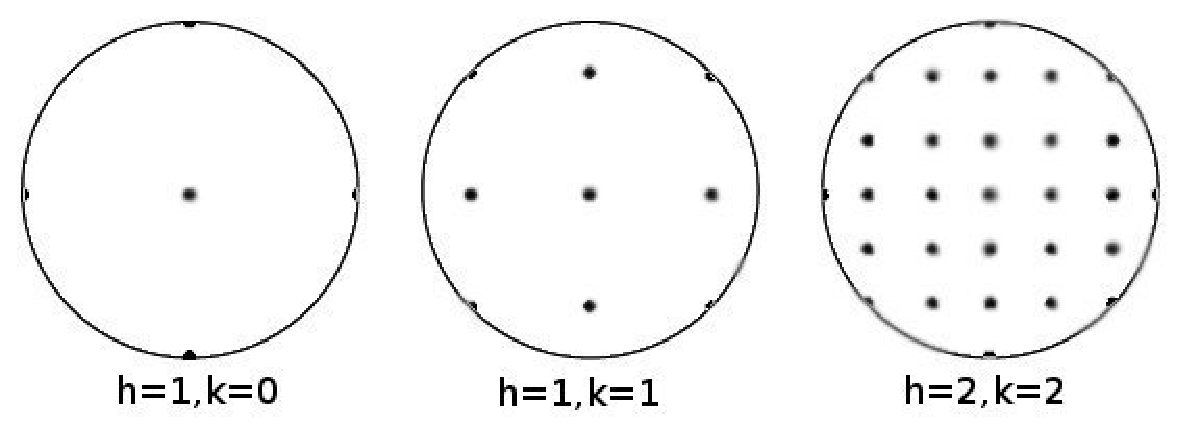
\includegraphics[scale=0.5]{img/reflexes}
\caption{Expected diffraction patterns for different energies \label{fig:reflexes}}
\end{figure}

\begin{table}
\begin{center}
\begin{tabular}{lcc}
\toprule
Reflex  & Energy\mbox{\,}[eV] at $\theta=45$\textdegree & Energy\mbox{\,}[eV] at $\theta=52$\textdegree \\
\midrule
(0,1) & \phantom{0}46.23 & \phantom{0}37.22 \\
(1,1) & \phantom{0}92.46 & \phantom{0}74.45 \\
(2,2) & 369.84 & 297.80 \\
\bottomrule
\end{tabular}
\end{center}
\par
\caption{Required electron energies for certain reflexes \label{tab:reqenerg}}
\end{table}

\subsection{Superstructures}

In our experiment we will adsorb oxygen O$_2$ on the copper surface we will examine. The oxygen will form a regular lattice structure on top of the copper surface---a so-called ($\sqrt{2} \times \sqrt{2}$)R$45$\textdegree superstructure. This superstructure notation, due to Woods, means that the lattice of the superstruce is obtained by scaling the x-direction by a factor of $\sqrt{2}$ and the y-direction by a factor of $2\sqrt{2}$ and rotating the lattice then by $45$\textdegree.

The superstructure will change the reciprocal latticr constants accordingly: $\tfrac{2\pi}{\sqrt{2}a}$  in the x- and $\tfrac{2\pi}{2\sqrt{2}a}$ y-direction.

The superstructure will also introduce a structure factor, since the unit cell is not now more complicated, which will make the former copper peaks stronger. 

\begin{figure}
\centering
\subfigure[ ]{
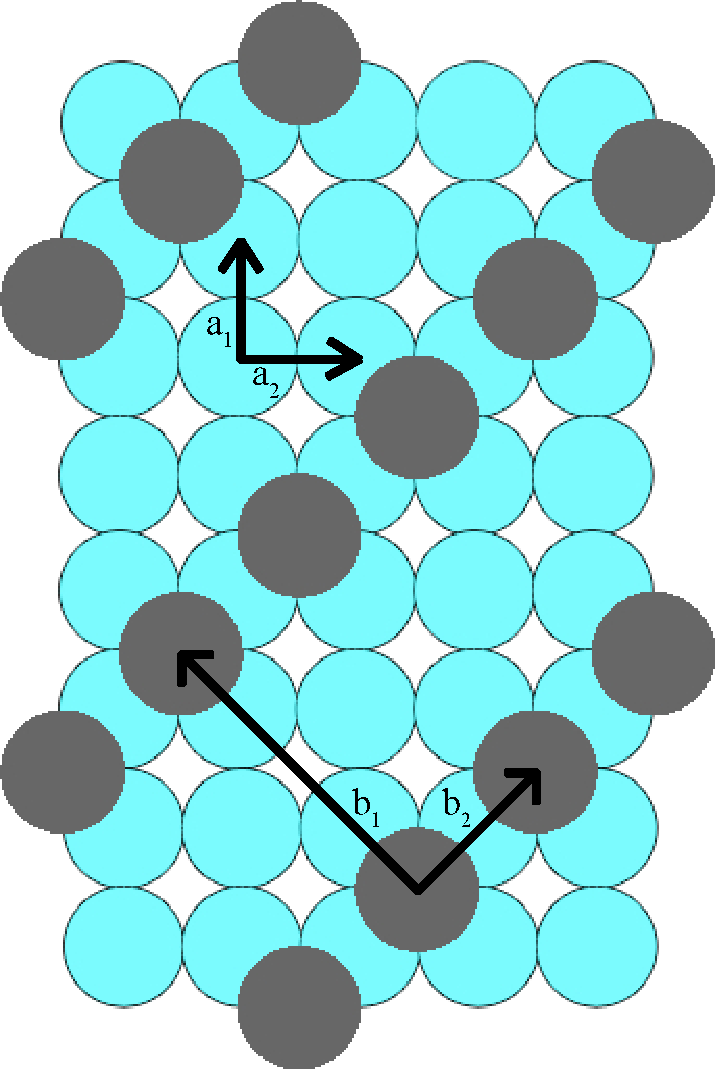
\includegraphics[scale=0.35]{img/superstructure1}
\label{fig:sup1}
}
\subfigure[ ]{
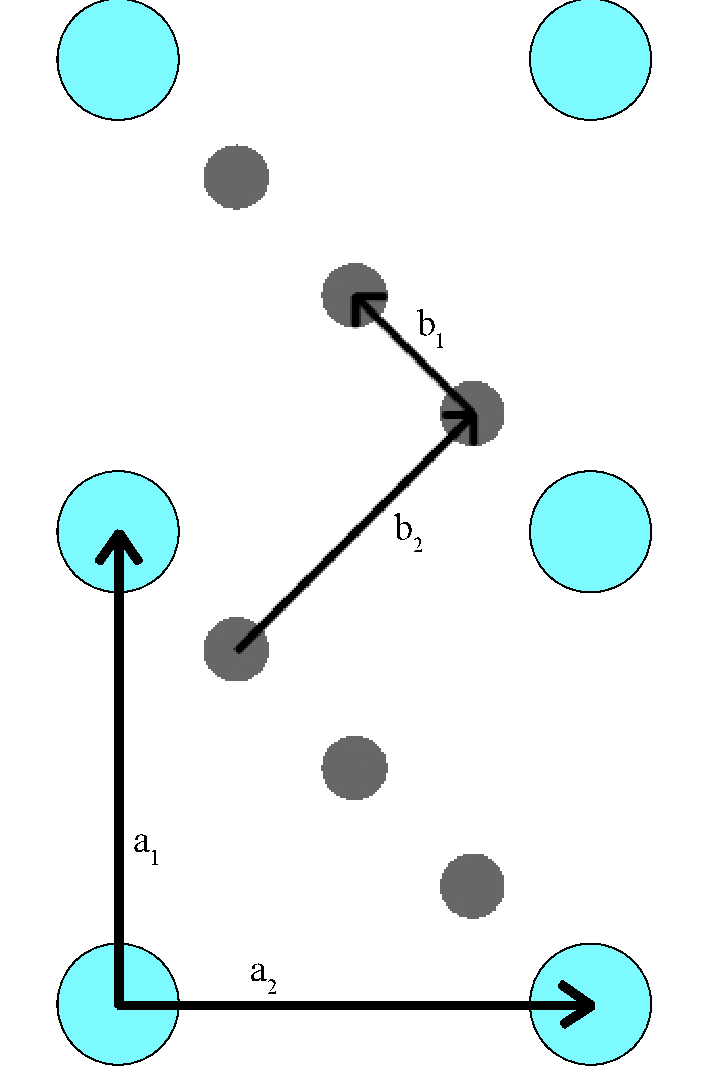
\includegraphics[scale=0.35]{img/superstructure2}
\label{fig:sup2}
}
\caption{The blue lattice in \subref{fig:sup1} is the regular lattice with lattice vectors $a_i$ and the grey lattice shows the ($\sqrt{2} \times \sqrt{2}$)R$45$\textdegree superstructure with lattice vectors $b_i$, \subref{fig:sup2} shows the same lattice in reciprocal space.}
\end{figure}

\subsection{Kinematic Approximation}

LEED can also be used to investigate the perpendicular lattice constant. Since the electrons need to penetrate the first lattice layer of the lattice and enter a strong potential, the simple model excluding multiple scattering events needs to be modified. We first modify equation~\eqref{eq:broglie1}
\begin{equation}
\lambda = \frac{h}{p} = \frac{h}{\sqrt{2m(E_{kin}-V)}}
\end{equation}
to account for energy loss in the scattering events. We will approximate $V$ as a constant potential. Using the above redefinition the perpendicular lattice constant is given by
\begin{equation}
2a_{\perp} = n\lambda = n \sqrt{\frac{h^{2}}{2m(E_{kin}-V)}}.
\end{equation}

\end{document}
